\documentclass[sigplan,screen]{acmart}
\settopmatter{printccs=false, printacmref=false}

\setcopyright{none}
\acmPrice{}
\acmDOI{}
\acmYear{}
\copyrightyear{}
\acmISBN{}
\acmConference[FARM '22]{Proceedings of the 10th ACM SIGPLAN International Workshop on Functional Art, Music, Modeling, and Design}{September 15, 2022}{Ljubljana, Slovenia}
\acmBooktitle{}

%% Bibliography style
\bibliographystyle{ACM-Reference-Format}
%% Citation style
%% Note: author/year citations are required for papers published as an
%% issue of PACMPL.
\citestyle{acmauthoryear}   %% For author/year citations

%% Some recommended packages.
\usepackage{booktabs}   %% For formal tables:
                        %% http://ctan.org/pkg/booktabs
\usepackage{subcaption} %% For complex figures with subfigures/subcaptions
                        %% http://ctan.org/pkg/subcaption
\usepackage{alltt}

\begin{document}

%% Title information
\title{Demo: Counterpoint Analysis and Synthesis}
%\subtitle{Functional Pearl}

%% Author information
%% Contents and number of authors suppressed with 'anonymous'.

\author{John Leo}
\affiliation{
  \institution{Halfaya Research}
  \city{Bellevue}
  \state{WA}
  \country{USA}
}
\email{leo@halfaya.org}


%% Abstract
%% Note: \begin{abstract}...\end{abstract} environment must come
%% before \maketitle command
\begin{abstract}
We present an Agda library to help analyze
and synthesize musical counterpoint. The tool allows expression of
generic constraints in a higher-level musical language which are
translated to a lower level for use both to find rule violations in
existing music and to generate (using an SMT solver) new
music satisfying the constraints. The tool is intended for use by
musicians who need only have a basic knowledge of Agda.
\end{abstract}


%% 2012 ACM Computing Classification System (CSS) concepts
%% Generate at 'http://dl.acm.org/ccs/ccs.cfm'.
\begin{CCSXML}
<ccs2012>
<concept>
<concept_id>10010405.10010469.10010475</concept_id>
<concept_desc>Applied computing~Sound and music computing</concept_desc>
<concept_significance>500</concept_significance>
</concept>
<concept>
<concept_id>10011007.10011006.10011008.10011009.10011012</concept_id>
<concept_desc>Software and its engineering~Functional languages</concept_desc>
<concept_significance>500</concept_significance>
</concept>
</ccs2012>
\end{CCSXML}

\ccsdesc[500]{Applied computing~Sound and music computing}
\ccsdesc[500]{Software and its engineering~Functional languages}
%% End of generated code

%% Keywords
%% comma separated list
\keywords{Counterpoint, Agda, SMT}  %% \keywords are mandatory in final camera-ready submission


%% \maketitle
%% Note: \maketitle command must come after title commands, author
%% commands, abstract environment, Computing Classification System
%% environment and commands, and keywords command.
\maketitle

\section{Introduction}

We demonstrate work in progress on a tool to assist in the analysis and
synthesis of musical counterpoint. Since the mid-18th century, the
composition of counterpoint has been guided by principles enunciated
in Fux's \textit{Gradus ad Parnassum} \citep{Fux1965}, first published
in 1725. Fux presents an increasingly sophisticated series of
``species'' (one note against one note, two notes against one note,
etc.) along with rules governing intervals between notes and motion
between intervals designed to ensure consonance and independence of
voices. It is well documented \citep{Mann1987} that composers
including Haydn, Mozart and Beethoven both studied and taught from
this text, and its fundamentals continue to be taught to music students
today (for example \cite{Kennan1999, Aldwell2018}).

In previous work, Cong and Leo \citep{CongLeo2019} encode the rules of
first-species (note against note) counterpoint as type constructors in
the dependently-typed language Agda. This enforces
correct-by-construction counterpoint and allows use of the Agda
typechecker to return errors with no additional effort required. On
the down side, these errors can be difficult to interpret for those
less familiar with type errors. Furthermore, encoding rules into
constructors is awkward for handling more complex species and more
global constraints. One could separate the construction of the pure
music from the constraints which can be added as a local or global
predicate (as in refinement types), but one may also wish to
deliberately violate some of the rules of strict counterpoint, as
composers often do in practice, and simply be informed of where the
violations occur without being prohibited from incorporating them.

Another approach then is to write a special-purpose ``type checker''
which can be run on previously-created music and which can generate
clear and precise error messages which are musically meaningful. The
checker is ideally easily customizable in terms of what constraints
one would like to impose. It turns out these constraints can be
expressed (at a low level) in the quantifier-free logic of linear
arithmetic and uninterpreted functions (QF-UFLIA \cite{Barrett2010}),
which allows one to not only analyze existing counterpoint, but also
synthesize counterpoint satisfying the constraints using an SMT
(Satisfiablity Modulo Theories) solver.

The initial prototype \citep{HaskellCounterpoint} of this tool was
written in Haskell, chosen due to the availability of the
high-quality and feature-rich SMT library SBV \citep{SBV}. It was then
ported to the Agda Music Tools library \cite{MusicTools}, using Agda's
Haskell foreign function interface (FFI) to call SBV. There is also an
Agda interface \citep{Schmitty} to SMT; we might convert to using
that at some point in the future.

The following sections give an overview of current
functionality. 

\section{An Example}

We briefly describe one way in which this tool can be used for both
analysis and synthesis. We first examine the example numbered 146 in
the critical edition of Beethoven's studies with Haydn
(\cite{BeethovenWerke13}; see also \cite{Nottebohm1971}, p.\ 31 and
\cite{Mann1987}, p.\ 115). It is shown in modern notation in
Figure~\ref{fig:b146}.

\begin{figure}
  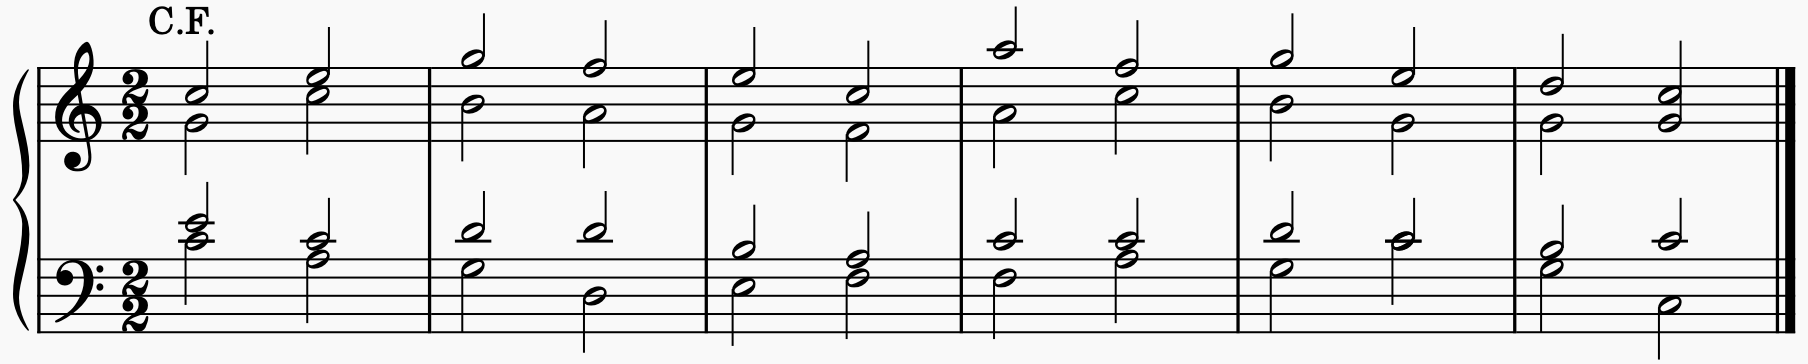
\includegraphics[width=8cm]{figures/b146.png}
  \caption{Beethoven Exercise 146}
  \Description{Beethoven Exercise 146}
  \label{fig:b146}
\end{figure}

Here Haydn has supplied the top voice, marked ``C.F.'' for cantus
firmus, and Beethoven's task was to supply the remaining three voices
following first species counterpoint rules. He uses only tones from
triads, all of them complete save the last and all in root position
save the second triad in bar 4. Since the notes form triads they
automatically satisfy consonance rules (only perfect intervals, thirds
or sixths between any pair of notes vertically); note that a perfect
fourth is prohibited in strict two part counterpoint but allowed with
more voices. Perfect fourths can be found between the top two voices
in the first, fourth and last bars.

There are boundary rules that the top and bottom voices must form
octaves at the beginning and end, and motion rules which are designed
to ensure independence of voices. In particular parallel and similar
(both voices moving in the same direction) motion into fifths and
octaves is prohibited. Here we can see that Beethoven has in fact made
two errors in the top two voices: similar motion into a fifth in bar 3
and then into an octave between bars 3 and 4. Haydn fixes both errors
by changing the F in the second voice (marked with the red X) to an A.

For simplicity we now focus only on the top two voices. Feeding
Beethoven's notes into the tool as two part first species
counterpoint, it easily finds and reports errors in the use of perfect
fourths, missing octaves at the boundaries, and similar motion into
fifths and octaves. We can disable the boundary rules as they are not
relevant and relax the consonance rule to allow perfect fourths, leaving
only the motion errors. We can replace the note F that Haydn fixed
with a hole, and run the tool in synthesis mode using the same
rules. It makes the same fix Haydn did. Perhaps we gave it too much
guidance, so instead we can create three holes in a row near the
error, which generates the solution shown in
Figure~\ref{fig:b146fix3}, with the three synthesized notes inside the
blue box. The only difference with Haydn's correction is
that the first note was changed from G to A as well. Although this
creates a satisfying oblique motion into a perfect fifth between bars
2 and 3, this same motion occurs between bars 5 and 6; furthermore we
now have four A notes in a row in addition to the three G notes at the
end of the second voice. For a middle voice this is not too bad, but
viewed as just two voices it is a bit dull.

\begin{figure}
  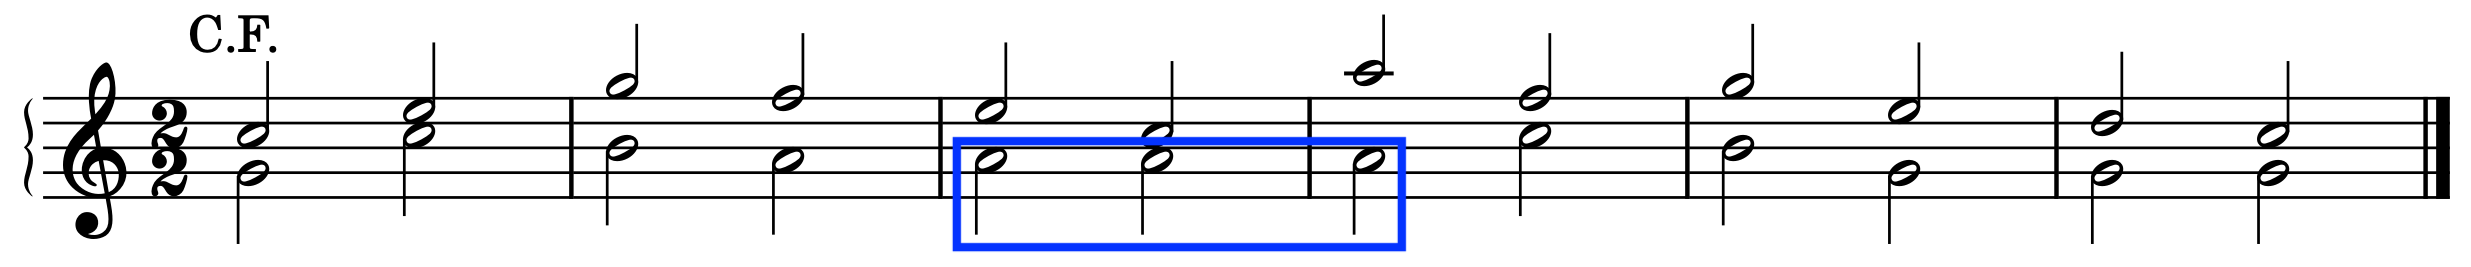
\includegraphics[width=8cm]{figures/b146fix3.png}
  \caption{Three Notes Synthesized}
  \Description{Three Notes Synthesized}
  \label{fig:b146fix3}
\end{figure}

This can be fixed by adding a constraint to limit the number of repeated
notes, but we can also try generating our own two part counterpoint
following Haydn's cantus firmus, fixing only the first and last of
Beethoven's notes. To help create better quality counterpoint we add
constraints to limit the number of leaps (horizontal intervals of more
than a major third) to at most one and require at least six instances
of contrary motion, which turns out to be maximal. We also disallow
perfect fourths except at the boundary. Note that it would
be extremely difficult for a human being with no computer assistance
to generate counterpoint following such restrictions, but the SMT
solver instantly returns the solution shown in
Figure~\ref{fig:b146gen3}. Contrary motion is shown by pairs of blue
arrows and the single leap by a red line.

\begin{figure}
  
\includegraphics[width=8cm]{figures/b146gen.png}
  \caption{Generated Counterpoint}
  \Description{Generated Counterpoint}
  \label{fig:b146gen3}
\end{figure}


\section{Selected Features}

We describe at a high level some of the key features of the
library; it is under development so details may change. The
latest code is available at \citep{MusicTools}.

The core component is a simple constraint language (\texttt{Expr}) of
booleans and integers. All constraints must be expressed at a low level
in this language. Integers represent absolute pitches and there are
named variables for synthesized pitches. Integer functions include
addition, subtraction and modulo. Equalities and inequalities convert
from integers to booleans; a monomorphic \texttt{if\_then\_else\_} allows
the reverse.

At a higher level, constraints (\texttt{Constraint}) are represented as
simple algebraic data types. For example \texttt{contrary}
denotes the \texttt{MotionConstraint} that two pairs of pitches
(each representing an vertical interval) represent contrary
motion. Constraints are compiled into boolean expressions, and only the
constraint author needs to understand these details; the user can
employ the high-level constraints directly.

At a higher level still, counterpoint rules (\texttt{Counterpoint})
take music as input and generate a list of constraints. For analysis of
music (no unknown pitches), constraints can be compiled and evaluated;
those which evaluate to false fail to hold. This can be done
interactively within emacs, for example.

For synthesis, the code must currently be compiled and run. The Agda
constraint language is converted to Haskell and compiled into symbolic
integers and booleans using SBV (\texttt{Smt}). An SMT solver
(currently only Z3 is supported) is called to solve for the variable
pitches, if possible. The result is then output as MIDI
(\texttt{SmtInterface}) which can then be opened and viewed with
notation software such as MuseScore.

\section{Future Plans}

Future plans include possible integration with Liquid Haskell
\citep{LiquidHaskell} (for analysis) and Synquid \citep{Synquid} (for
synthesis). In addition to handling higher species we would like to
also incorporate the rules and conventions of galant schemata
\citep{Gjerdingen2007}, which informed much of the music composed in
the era of Haydn and Mozart. Ideally one could use the tool to compose
convincing music in the galant style.

Concurrently Cong \citep{Cong2022a,Cong2022c} is exploring another approach
using a different representation of constraints within a type system.
Recent work by Tanaka \citep{Tanaka2022} uses integer programming to
express constraints, and we plan to compare our method with this.

\section*{Acknowledgements}

Thanks to Youyou Cong for many enlightening discussions about type
theory and music over the past several years, and for suggesting to
look at Beethoven's exercises as a source of examples. Thanks also to
Emina Torlak and Stephen Rumph for their generosity in allowing me to
audit their classes at the University of Washington. CSE 507 was
invaluable for learning the fundamentals of SMT 
solvers, and MUHST 211 and 430 introduced me to galant schemata.
Finally, thanks the anonymous referees for many helpful comments and
suggestions.

%% Bibliography
\bibliography{abstract.bib}

\end{document}
